\ifdefined\ICLRLayout
\clearpage
% 中文版保留原始数值与方法名称。
\definecolor{tabaceSharedRow}{HTML}{EAF4FB}
\definecolor{tabaceSpecificRow}{HTML}{FFF4D6}
\definecolor{tabaceSharedText}{HTML}{0072B2}
\definecolor{tabaceSpecificText}{HTML}{D55E00}
\ifdefined\ICLRLayout
\begin{table}[H]
\else
\begin{table}[H]
\fi
  \caption{OpenML-CC18 分类与 OpenML-CTR23 回归任务上的整体性能。扰动和偏移区块分别在五种和七种变化类别的全部非零强度上进行宏平均。}
  \label{tab:overall-performance}
  \centering
  \scriptsize
  \setlength{\tabcolsep}{2.0pt}
  \renewcommand{\arraystretch}{0.98}
  \begin{tabular}{@{}l*{12}{c}@{}}
    \toprule
    & \multicolumn{4}{c}{干净数据}
    & \multicolumn{4}{c}{五种扰动（平均）}
    & \multicolumn{4}{c}{七种偏移（平均）} \\
    \cmidrule(lr){2-5}\cmidrule(lr){6-9}\cmidrule(lr){10-13}
    & \multicolumn{2}{c}{分类} & \multicolumn{2}{c}{回归}
    & \multicolumn{2}{c}{分类} & \multicolumn{2}{c}{回归}
    & \multicolumn{2}{c}{分类} & \multicolumn{2}{c}{回归} \\
    \cmidrule(lr){2-3}\cmidrule(lr){4-5}
    \cmidrule(lr){6-7}\cmidrule(lr){8-9}
    \cmidrule(lr){10-11}\cmidrule(lr){12-13}
    方法
    & Acc$\uparrow$ & AUC$\uparrow$ & $R^2\uparrow$ & nRMSE$\downarrow$
    & Acc$\uparrow$ & AUC$\uparrow$ & $R^2\uparrow$ & nRMSE$\downarrow$
    & Acc$\uparrow$ & AUC$\uparrow$ & $R^2\uparrow$ & nRMSE$\downarrow$ \\
    \midrule
    \multicolumn{13}{@{}l}{\textit{非 TFM 基线}} \\
    LogReg/Ridge + HPO & 0.754 & 0.867 & 0.543 & 0.684 & 0.418 & 0.582 & -0.559 & 1.175 & 0.719 & 0.775 & -0.490 & 0.851 \\
    SVM/SVR + HPO & 0.777 & 0.879 & 0.492 & 0.703 & 0.449 & 0.611 & -0.872 & 1.255 & 0.757 & 0.793 & 0.010 & 0.873 \\
    kNN + HPO & 0.726 & 0.856 & 0.587 & 0.656 & 0.489 & 0.647 & -1.245 & 1.396 & 0.743 & 0.775 & 0.327 & 0.779 \\
    RF + HPO & 0.776 & 0.886 & 0.676 & 0.561 & 0.451 & 0.649 & -1.218 & 1.335 & 0.760 & 0.810 & 0.385 & 0.724 \\
    LightGBM + HPO & 0.776 & 0.884 & 0.697 & 0.529 & 0.463 & 0.639 & -1.215 & 1.337 & 0.759 & 0.796 & 0.350 & 0.736 \\
    CatBoost + HPO & 0.782 & 0.890 & 0.708 & 0.514 & 0.479 & 0.653 & -1.372 & 1.368 & 0.770 & 0.811 & 0.381 & 0.711 \\
    XGBoost + HPO & 0.774 & 0.885 & 0.702 & 0.525 & 0.455 & 0.640 & -1.323 & 1.359 & 0.751 & 0.796 & 0.278 & 0.767 \\
    MLP + HPO & 0.729 & 0.858 & 0.583 & 0.568 & 0.435 & 0.604 & -1.007 & 1.272 & 0.741 & 0.767 & 0.066 & 0.828 \\
    FT-Transformer & 0.745 & 0.861 & 0.657 & 0.568 & 0.456 & 0.619 & -1.256 & 1.353 & 0.716 & 0.765 & 0.210 & 0.822 \\
    TabM & 0.735 & 0.866 & 0.655 & 0.577 & 0.454 & 0.614 & -1.100 & 1.324 & 0.699 & 0.743 & 0.212 & 0.811 \\
    TabulaRNN & 0.722 & 0.856 & 0.580 & 0.648 & 0.454 & 0.625 & -0.851 & 1.270 & 0.718 & 0.754 & 0.205 & 0.845 \\
    MambaTab & 0.748 & 0.869 & 0.663 & 0.564 & 0.434 & 0.602 & -0.824 & 1.230 & 0.751 & 0.784 & 0.279 & 0.761 \\
    RealMLP & 0.762 & 0.872 & 0.694 & 0.527 & 0.448 & 0.614 & -1.258 & 1.326 & 0.758 & 0.793 & 0.240 & 0.749 \\
    \midrule
    LimiX-2M & 0.796 & 0.896 & 0.724 & 0.494 & 0.475 & 0.657 & -1.141 & 1.277 & 0.781 & 0.831 & 0.385 & 0.689 \\
    \rowcolor{tabaceSharedRow}
    \textcolor{tabaceSharedText}{\textbf{+ \method{}-shared}} & \textcolor{tabaceSharedText}{\textbf{0.796}} & \textcolor{tabaceSharedText}{\textbf{0.896}} & \textcolor{tabaceSharedText}{\textbf{0.725}} & \textcolor{tabaceSharedText}{\textbf{0.493}} & \textcolor{tabaceSharedText}{\textbf{0.542}} & \textcolor{tabaceSharedText}{\textbf{0.716}} & \textcolor{tabaceSharedText}{\textbf{-0.173}} & \textcolor{tabaceSharedText}{\textbf{1.059}} & \textcolor{tabaceSharedText}{\textbf{0.784}} & \textcolor{tabaceSharedText}{\textbf{0.835}} & \textcolor{tabaceSharedText}{\textbf{0.498}} & \textcolor{tabaceSharedText}{\textbf{0.659}} \\
    \rowcolor{tabaceSpecificRow}
    \textcolor{tabaceSpecificText}{\textbf{+ \method{}-specific}} & \textcolor{tabaceSpecificText}{\textbf{0.796}} & \textcolor{tabaceSpecificText}{\textbf{0.896}} & \textcolor{tabaceSpecificText}{\textbf{0.725}} & \textcolor{tabaceSpecificText}{\textbf{0.493}} & \textcolor{tabaceSpecificText}{\textbf{0.628}} & \textcolor{tabaceSpecificText}{\textbf{0.769}} & \textcolor{tabaceSpecificText}{\textbf{0.053}} & \textcolor{tabaceSpecificText}{\textbf{0.947}} & \textcolor{tabaceSpecificText}{\textbf{0.804}} & \textcolor{tabaceSpecificText}{\textbf{0.847}} & \textcolor{tabaceSpecificText}{\textbf{0.629}} & \textcolor{tabaceSpecificText}{\textbf{0.563}} \\
    \midrule
    TabICL-v2 & 0.804 & 0.901 & 0.739 & 0.476 & 0.494 & 0.676 & -1.077 & 1.270 & 0.763 & 0.826 & 0.273 & 0.730 \\
    \rowcolor{tabaceSharedRow}
    \textcolor{tabaceSharedText}{\textbf{+ \method{}-shared}} & \textcolor{tabaceSharedText}{\textbf{0.804}} & \textcolor{tabaceSharedText}{\textbf{0.901}} & \textcolor{tabaceSharedText}{\textbf{0.738}} & \textcolor{tabaceSharedText}{\textbf{0.478}} & \textcolor{tabaceSharedText}{\textbf{0.575}} & \textcolor{tabaceSharedText}{\textbf{0.720}} & \textcolor{tabaceSharedText}{\textbf{0.363}} & \textcolor{tabaceSharedText}{\textbf{0.783}} & \textcolor{tabaceSharedText}{\textbf{0.772}} & \textcolor{tabaceSharedText}{\textbf{0.831}} & \textcolor{tabaceSharedText}{\textbf{0.467}} & \textcolor{tabaceSharedText}{\textbf{0.659}} \\
    \rowcolor{tabaceSpecificRow}
    \textcolor{tabaceSpecificText}{\textbf{+ \method{}-specific}} & \textcolor{tabaceSpecificText}{\textbf{0.804}} & \textcolor{tabaceSpecificText}{\textbf{0.900}} & \textcolor{tabaceSpecificText}{\textbf{0.738}} & \textcolor{tabaceSpecificText}{\textbf{0.476}} & \textcolor{tabaceSpecificText}{\textbf{0.610}} & \textcolor{tabaceSpecificText}{\textbf{0.752}} & \textcolor{tabaceSpecificText}{\textbf{0.485}} & \textcolor{tabaceSpecificText}{\textbf{0.708}} & \textcolor{tabaceSpecificText}{\textbf{0.805}} & \textcolor{tabaceSpecificText}{\textbf{0.854}} & \textcolor{tabaceSpecificText}{\textbf{0.655}} & \textcolor{tabaceSpecificText}{\textbf{0.535}} \\
    \midrule
    TabPFN-v3 & 0.793 & 0.893 & 0.739 & 0.476 & 0.457 & 0.636 & -1.253 & 1.313 & 0.758 & 0.809 & 0.426 & 0.669 \\
    \rowcolor{tabaceSharedRow}
    \textcolor{tabaceSharedText}{\textbf{+ \method{}-shared}} & \textcolor{tabaceSharedText}{\textbf{0.792}} & \textcolor{tabaceSharedText}{\textbf{0.893}} & \textcolor{tabaceSharedText}{\textbf{0.739}} & \textcolor{tabaceSharedText}{\textbf{0.480}} & \textcolor{tabaceSharedText}{\textbf{0.553}} & \textcolor{tabaceSharedText}{\textbf{0.697}} & \textcolor{tabaceSharedText}{\textbf{0.237}} & \textcolor{tabaceSharedText}{\textbf{0.834}} & \textcolor{tabaceSharedText}{\textbf{0.770}} & \textcolor{tabaceSharedText}{\textbf{0.817}} & \textcolor{tabaceSharedText}{\textbf{0.460}} & \textcolor{tabaceSharedText}{\textbf{0.656}} \\
    \rowcolor{tabaceSpecificRow}
    \textcolor{tabaceSpecificText}{\textbf{+ \method{}-specific}} & \textcolor{tabaceSpecificText}{\textbf{0.792}} & \textcolor{tabaceSpecificText}{\textbf{0.893}} & \textcolor{tabaceSpecificText}{\textbf{0.739}} & \textcolor{tabaceSpecificText}{\textbf{0.477}} & \textcolor{tabaceSpecificText}{\textbf{0.593}} & \textcolor{tabaceSpecificText}{\textbf{0.739}} & \textcolor{tabaceSpecificText}{\textbf{0.588}} & \textcolor{tabaceSpecificText}{\textbf{0.635}} & \textcolor{tabaceSpecificText}{\textbf{0.788}} & \textcolor{tabaceSpecificText}{\textbf{0.835}} & \textcolor{tabaceSpecificText}{\textbf{0.620}} & \textcolor{tabaceSpecificText}{\textbf{0.565}} \\
    \midrule
    TabDPT v1.2 & 0.779 & 0.891 & 0.731 & 0.488 & 0.448 & 0.631 & -1.152 & 1.300 & 0.774 & 0.821 & 0.514 & 0.633 \\
    \rowcolor{tabaceSharedRow}
    \textcolor{tabaceSharedText}{\textbf{+ \method{}-shared}} & \textcolor{tabaceSharedText}{\textbf{0.779}} & \textcolor{tabaceSharedText}{\textbf{0.891}} & \textcolor{tabaceSharedText}{\textbf{0.730}} & \textcolor{tabaceSharedText}{\textbf{0.491}} & \textcolor{tabaceSharedText}{\textbf{0.548}} & \textcolor{tabaceSharedText}{\textbf{0.694}} & \textcolor{tabaceSharedText}{\textbf{0.329}} & \textcolor{tabaceSharedText}{\textbf{0.803}} & \textcolor{tabaceSharedText}{\textbf{0.781}} & \textcolor{tabaceSharedText}{\textbf{0.831}} & \textcolor{tabaceSharedText}{\textbf{0.547}} & \textcolor{tabaceSharedText}{\textbf{0.614}} \\
    \rowcolor{tabaceSpecificRow}
    \textcolor{tabaceSpecificText}{\textbf{+ \method{}-specific}} & \textcolor{tabaceSpecificText}{\textbf{0.779}} & \textcolor{tabaceSpecificText}{\textbf{0.891}} & \textcolor{tabaceSpecificText}{\textbf{0.730}} & \textcolor{tabaceSpecificText}{\textbf{0.488}} & \textcolor{tabaceSpecificText}{\textbf{0.600}} & \textcolor{tabaceSpecificText}{\textbf{0.746}} & \textcolor{tabaceSpecificText}{\textbf{0.443}} & \textcolor{tabaceSpecificText}{\textbf{0.733}} & \textcolor{tabaceSpecificText}{\textbf{0.805}} & \textcolor{tabaceSpecificText}{\textbf{0.846}} & \textcolor{tabaceSpecificText}{\textbf{0.610}} & \textcolor{tabaceSpecificText}{\textbf{0.572}} \\
    \bottomrule
  \end{tabular}
\ifdefined\ICLRLayout
\end{table}
\else
\end{table}
\fi

\else
\begin{figure}[H]
  \centering
  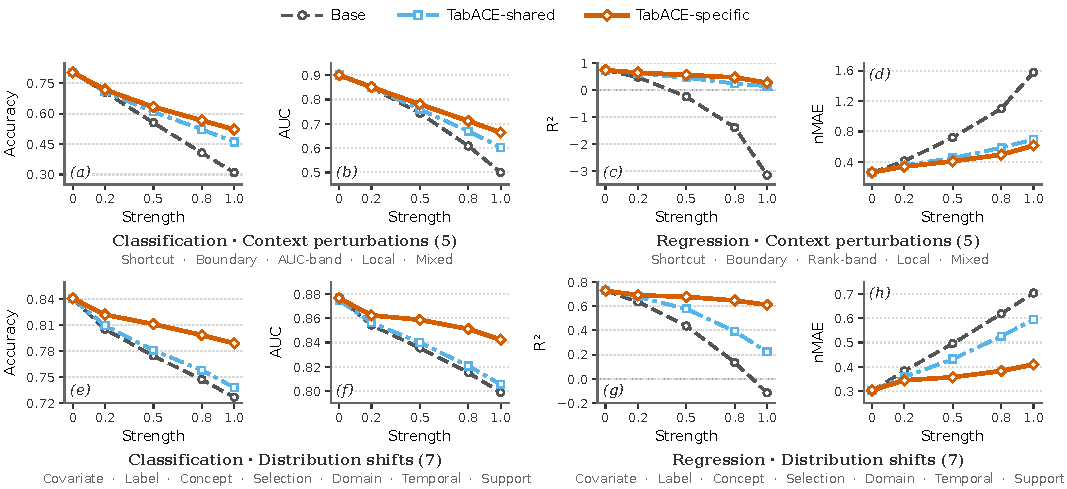
\includegraphics[width=\textwidth]{figures/tabace_strength_comparison.pdf}
  \caption{OpenML 基准上不同问题强度下的性能。分类面板使用 OpenML-CC18，回归面板使用 OpenML-CTR23。第一行对五种受控上下文扰动进行宏平均，第二行对七种分布偏移进行宏平均。}
  \label{fig:semisynthetic-strength}
\end{figure}

\clearpage
% 中文版保留原始数值与方法名称。
\definecolor{tabaceSharedRow}{HTML}{EAF4FB}
\definecolor{tabaceSpecificRow}{HTML}{FFF4D6}
\definecolor{tabaceSharedText}{HTML}{0072B2}
\definecolor{tabaceSpecificText}{HTML}{D55E00}
\ifdefined\ICLRLayout
\begin{table}[H]
\else
\begin{table}[H]
\fi
  \caption{OpenML-CC18 分类与 OpenML-CTR23 回归任务上的整体性能。扰动和偏移区块分别在五种和七种变化类别的全部非零强度上进行宏平均。}
  \label{tab:overall-performance}
  \centering
  \scriptsize
  \setlength{\tabcolsep}{2.0pt}
  \renewcommand{\arraystretch}{0.98}
  \begin{tabular}{@{}l*{12}{c}@{}}
    \toprule
    & \multicolumn{4}{c}{干净数据}
    & \multicolumn{4}{c}{五种扰动（平均）}
    & \multicolumn{4}{c}{七种偏移（平均）} \\
    \cmidrule(lr){2-5}\cmidrule(lr){6-9}\cmidrule(lr){10-13}
    & \multicolumn{2}{c}{分类} & \multicolumn{2}{c}{回归}
    & \multicolumn{2}{c}{分类} & \multicolumn{2}{c}{回归}
    & \multicolumn{2}{c}{分类} & \multicolumn{2}{c}{回归} \\
    \cmidrule(lr){2-3}\cmidrule(lr){4-5}
    \cmidrule(lr){6-7}\cmidrule(lr){8-9}
    \cmidrule(lr){10-11}\cmidrule(lr){12-13}
    方法
    & Acc$\uparrow$ & AUC$\uparrow$ & $R^2\uparrow$ & nRMSE$\downarrow$
    & Acc$\uparrow$ & AUC$\uparrow$ & $R^2\uparrow$ & nRMSE$\downarrow$
    & Acc$\uparrow$ & AUC$\uparrow$ & $R^2\uparrow$ & nRMSE$\downarrow$ \\
    \midrule
    \multicolumn{13}{@{}l}{\textit{非 TFM 基线}} \\
    LogReg/Ridge + HPO & 0.754 & 0.867 & 0.543 & 0.684 & 0.418 & 0.582 & -0.559 & 1.175 & 0.719 & 0.775 & -0.490 & 0.851 \\
    SVM/SVR + HPO & 0.777 & 0.879 & 0.492 & 0.703 & 0.449 & 0.611 & -0.872 & 1.255 & 0.757 & 0.793 & 0.010 & 0.873 \\
    kNN + HPO & 0.726 & 0.856 & 0.587 & 0.656 & 0.489 & 0.647 & -1.245 & 1.396 & 0.743 & 0.775 & 0.327 & 0.779 \\
    RF + HPO & 0.776 & 0.886 & 0.676 & 0.561 & 0.451 & 0.649 & -1.218 & 1.335 & 0.760 & 0.810 & 0.385 & 0.724 \\
    LightGBM + HPO & 0.776 & 0.884 & 0.697 & 0.529 & 0.463 & 0.639 & -1.215 & 1.337 & 0.759 & 0.796 & 0.350 & 0.736 \\
    CatBoost + HPO & 0.782 & 0.890 & 0.708 & 0.514 & 0.479 & 0.653 & -1.372 & 1.368 & 0.770 & 0.811 & 0.381 & 0.711 \\
    XGBoost + HPO & 0.774 & 0.885 & 0.702 & 0.525 & 0.455 & 0.640 & -1.323 & 1.359 & 0.751 & 0.796 & 0.278 & 0.767 \\
    MLP + HPO & 0.729 & 0.858 & 0.583 & 0.568 & 0.435 & 0.604 & -1.007 & 1.272 & 0.741 & 0.767 & 0.066 & 0.828 \\
    FT-Transformer & 0.745 & 0.861 & 0.657 & 0.568 & 0.456 & 0.619 & -1.256 & 1.353 & 0.716 & 0.765 & 0.210 & 0.822 \\
    TabM & 0.735 & 0.866 & 0.655 & 0.577 & 0.454 & 0.614 & -1.100 & 1.324 & 0.699 & 0.743 & 0.212 & 0.811 \\
    TabulaRNN & 0.722 & 0.856 & 0.580 & 0.648 & 0.454 & 0.625 & -0.851 & 1.270 & 0.718 & 0.754 & 0.205 & 0.845 \\
    MambaTab & 0.748 & 0.869 & 0.663 & 0.564 & 0.434 & 0.602 & -0.824 & 1.230 & 0.751 & 0.784 & 0.279 & 0.761 \\
    RealMLP & 0.762 & 0.872 & 0.694 & 0.527 & 0.448 & 0.614 & -1.258 & 1.326 & 0.758 & 0.793 & 0.240 & 0.749 \\
    \midrule
    LimiX-2M & 0.796 & 0.896 & 0.724 & 0.494 & 0.475 & 0.657 & -1.141 & 1.277 & 0.781 & 0.831 & 0.385 & 0.689 \\
    \rowcolor{tabaceSharedRow}
    \textcolor{tabaceSharedText}{\textbf{+ \method{}-shared}} & \textcolor{tabaceSharedText}{\textbf{0.796}} & \textcolor{tabaceSharedText}{\textbf{0.896}} & \textcolor{tabaceSharedText}{\textbf{0.725}} & \textcolor{tabaceSharedText}{\textbf{0.493}} & \textcolor{tabaceSharedText}{\textbf{0.542}} & \textcolor{tabaceSharedText}{\textbf{0.716}} & \textcolor{tabaceSharedText}{\textbf{-0.173}} & \textcolor{tabaceSharedText}{\textbf{1.059}} & \textcolor{tabaceSharedText}{\textbf{0.784}} & \textcolor{tabaceSharedText}{\textbf{0.835}} & \textcolor{tabaceSharedText}{\textbf{0.498}} & \textcolor{tabaceSharedText}{\textbf{0.659}} \\
    \rowcolor{tabaceSpecificRow}
    \textcolor{tabaceSpecificText}{\textbf{+ \method{}-specific}} & \textcolor{tabaceSpecificText}{\textbf{0.796}} & \textcolor{tabaceSpecificText}{\textbf{0.896}} & \textcolor{tabaceSpecificText}{\textbf{0.725}} & \textcolor{tabaceSpecificText}{\textbf{0.493}} & \textcolor{tabaceSpecificText}{\textbf{0.628}} & \textcolor{tabaceSpecificText}{\textbf{0.769}} & \textcolor{tabaceSpecificText}{\textbf{0.053}} & \textcolor{tabaceSpecificText}{\textbf{0.947}} & \textcolor{tabaceSpecificText}{\textbf{0.804}} & \textcolor{tabaceSpecificText}{\textbf{0.847}} & \textcolor{tabaceSpecificText}{\textbf{0.629}} & \textcolor{tabaceSpecificText}{\textbf{0.563}} \\
    \midrule
    TabICL-v2 & 0.804 & 0.901 & 0.739 & 0.476 & 0.494 & 0.676 & -1.077 & 1.270 & 0.763 & 0.826 & 0.273 & 0.730 \\
    \rowcolor{tabaceSharedRow}
    \textcolor{tabaceSharedText}{\textbf{+ \method{}-shared}} & \textcolor{tabaceSharedText}{\textbf{0.804}} & \textcolor{tabaceSharedText}{\textbf{0.901}} & \textcolor{tabaceSharedText}{\textbf{0.738}} & \textcolor{tabaceSharedText}{\textbf{0.478}} & \textcolor{tabaceSharedText}{\textbf{0.575}} & \textcolor{tabaceSharedText}{\textbf{0.720}} & \textcolor{tabaceSharedText}{\textbf{0.363}} & \textcolor{tabaceSharedText}{\textbf{0.783}} & \textcolor{tabaceSharedText}{\textbf{0.772}} & \textcolor{tabaceSharedText}{\textbf{0.831}} & \textcolor{tabaceSharedText}{\textbf{0.467}} & \textcolor{tabaceSharedText}{\textbf{0.659}} \\
    \rowcolor{tabaceSpecificRow}
    \textcolor{tabaceSpecificText}{\textbf{+ \method{}-specific}} & \textcolor{tabaceSpecificText}{\textbf{0.804}} & \textcolor{tabaceSpecificText}{\textbf{0.900}} & \textcolor{tabaceSpecificText}{\textbf{0.738}} & \textcolor{tabaceSpecificText}{\textbf{0.476}} & \textcolor{tabaceSpecificText}{\textbf{0.610}} & \textcolor{tabaceSpecificText}{\textbf{0.752}} & \textcolor{tabaceSpecificText}{\textbf{0.485}} & \textcolor{tabaceSpecificText}{\textbf{0.708}} & \textcolor{tabaceSpecificText}{\textbf{0.805}} & \textcolor{tabaceSpecificText}{\textbf{0.854}} & \textcolor{tabaceSpecificText}{\textbf{0.655}} & \textcolor{tabaceSpecificText}{\textbf{0.535}} \\
    \midrule
    TabPFN-v3 & 0.793 & 0.893 & 0.739 & 0.476 & 0.457 & 0.636 & -1.253 & 1.313 & 0.758 & 0.809 & 0.426 & 0.669 \\
    \rowcolor{tabaceSharedRow}
    \textcolor{tabaceSharedText}{\textbf{+ \method{}-shared}} & \textcolor{tabaceSharedText}{\textbf{0.792}} & \textcolor{tabaceSharedText}{\textbf{0.893}} & \textcolor{tabaceSharedText}{\textbf{0.739}} & \textcolor{tabaceSharedText}{\textbf{0.480}} & \textcolor{tabaceSharedText}{\textbf{0.553}} & \textcolor{tabaceSharedText}{\textbf{0.697}} & \textcolor{tabaceSharedText}{\textbf{0.237}} & \textcolor{tabaceSharedText}{\textbf{0.834}} & \textcolor{tabaceSharedText}{\textbf{0.770}} & \textcolor{tabaceSharedText}{\textbf{0.817}} & \textcolor{tabaceSharedText}{\textbf{0.460}} & \textcolor{tabaceSharedText}{\textbf{0.656}} \\
    \rowcolor{tabaceSpecificRow}
    \textcolor{tabaceSpecificText}{\textbf{+ \method{}-specific}} & \textcolor{tabaceSpecificText}{\textbf{0.792}} & \textcolor{tabaceSpecificText}{\textbf{0.893}} & \textcolor{tabaceSpecificText}{\textbf{0.739}} & \textcolor{tabaceSpecificText}{\textbf{0.477}} & \textcolor{tabaceSpecificText}{\textbf{0.593}} & \textcolor{tabaceSpecificText}{\textbf{0.739}} & \textcolor{tabaceSpecificText}{\textbf{0.588}} & \textcolor{tabaceSpecificText}{\textbf{0.635}} & \textcolor{tabaceSpecificText}{\textbf{0.788}} & \textcolor{tabaceSpecificText}{\textbf{0.835}} & \textcolor{tabaceSpecificText}{\textbf{0.620}} & \textcolor{tabaceSpecificText}{\textbf{0.565}} \\
    \midrule
    TabDPT v1.2 & 0.779 & 0.891 & 0.731 & 0.488 & 0.448 & 0.631 & -1.152 & 1.300 & 0.774 & 0.821 & 0.514 & 0.633 \\
    \rowcolor{tabaceSharedRow}
    \textcolor{tabaceSharedText}{\textbf{+ \method{}-shared}} & \textcolor{tabaceSharedText}{\textbf{0.779}} & \textcolor{tabaceSharedText}{\textbf{0.891}} & \textcolor{tabaceSharedText}{\textbf{0.730}} & \textcolor{tabaceSharedText}{\textbf{0.491}} & \textcolor{tabaceSharedText}{\textbf{0.548}} & \textcolor{tabaceSharedText}{\textbf{0.694}} & \textcolor{tabaceSharedText}{\textbf{0.329}} & \textcolor{tabaceSharedText}{\textbf{0.803}} & \textcolor{tabaceSharedText}{\textbf{0.781}} & \textcolor{tabaceSharedText}{\textbf{0.831}} & \textcolor{tabaceSharedText}{\textbf{0.547}} & \textcolor{tabaceSharedText}{\textbf{0.614}} \\
    \rowcolor{tabaceSpecificRow}
    \textcolor{tabaceSpecificText}{\textbf{+ \method{}-specific}} & \textcolor{tabaceSpecificText}{\textbf{0.779}} & \textcolor{tabaceSpecificText}{\textbf{0.891}} & \textcolor{tabaceSpecificText}{\textbf{0.730}} & \textcolor{tabaceSpecificText}{\textbf{0.488}} & \textcolor{tabaceSpecificText}{\textbf{0.600}} & \textcolor{tabaceSpecificText}{\textbf{0.746}} & \textcolor{tabaceSpecificText}{\textbf{0.443}} & \textcolor{tabaceSpecificText}{\textbf{0.733}} & \textcolor{tabaceSpecificText}{\textbf{0.805}} & \textcolor{tabaceSpecificText}{\textbf{0.846}} & \textcolor{tabaceSpecificText}{\textbf{0.610}} & \textcolor{tabaceSpecificText}{\textbf{0.572}} \\
    \bottomrule
  \end{tabular}
\ifdefined\ICLRLayout
\end{table}
\else
\end{table}
\fi

\fi

\section{实验}
\label{sec:experiments}

\subsection{实验设置}
\label{sec:experimental_setup}

\paragraph{评估轨道。}
我们在公开 OpenML 基准和全合成数据上评估 TabACE。OpenML 轨道的分类任务来自 OpenML-CC18~\citep{bischl2021openml}，回归任务来自 OpenML-CTR23~\citep{fischer2023openmlctr23}。受控变化采用五折数据集级折外（OOF）评估：策略在其余四折上拟合，并在留出数据集上保持固定。强度为零时，上下文与输入均不改变。合成轨道使用受控数据生成过程，分别考察问题类别与强度的影响。

\paragraph{问题与配置。}
两个轨道均覆盖五种源上下文扰动（Shortcut、Boundary、AUC/Rank-band、Local 和 Mixed）与七种分布偏移（Covariate、Label、Concept、Selection、Domain、Temporal 和 Support），强度取 $0$、$0.2$、$0.5$、$0.8$ 和 $1.0$。Base 表示不进行上下文集成的冻结主干模型。Shared 在所有预定义变化上采用固定上下文库；Specific 则根据目标推理前给定的变化类别选择并融合候选上下文。除非另行注明预测器，所有次要实验均采用冻结的 TabICL-v2，Base 表示其未经修改的预测。附录列出全部算子与上下文布局。

% Register this float before the final setup paragraphs so that the arXiv
% layout places it at the top of page 7.  The ICLR layout inserts the same
% figure at the corresponding results subsection instead.
\ifdefined\ICLRLayout\else
\clearpage
\begin{figure}[H]
  \centering
  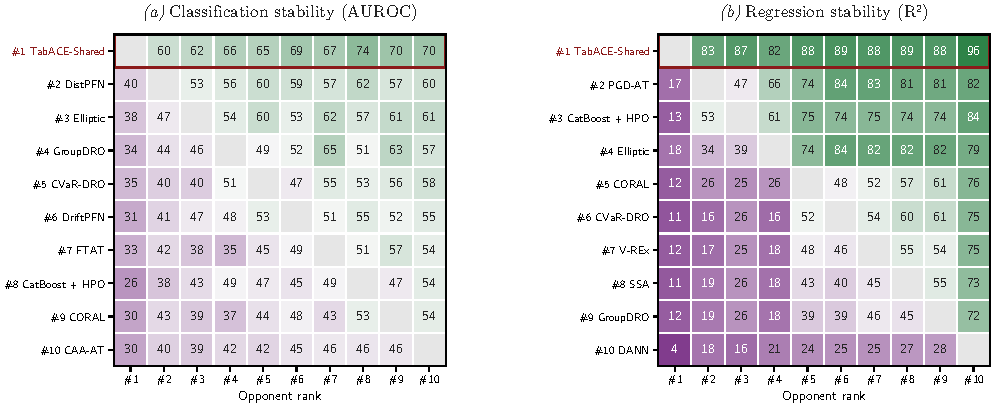
\includegraphics[width=0.88\textwidth]{figures/tabace_synthetic_stability.pdf}
  \caption{在 180 个对齐的“随机种子--DGP--场景”实验单元上的成对稳定性。分类使用经机会水平校正的 AUROC 边际退化，回归使用归一化 $R^2$ 退化。单元格表示行方法取得较小性能下降的频率；差异不超过 $0.001$ 时记为平局。}
  \label{fig:synthetic-stability}
\end{figure}

\begin{figure}[H]
  \centering
  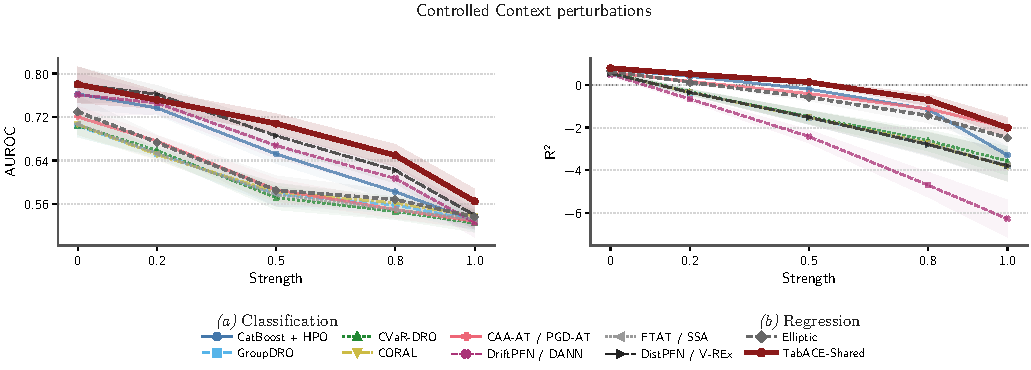
\includegraphics[width=0.94\textwidth]{figures/tabace_controlled_response.pdf}
  \caption{全合成设置下对受控上下文扰动的响应。各面板分别报告分类 AUROC 与回归 $R^2$；曲线汇总五种扰动类别上的对齐实验单元，阴影带表示 $95\%$ bootstrap 区间。}
  \label{fig:synthetic-controlled-response}
\end{figure}
\fi

\paragraph{任务与指标。}
分类任务报告 Accuracy 和 AUROC，回归任务报告 $R^2$、nMAE 与 nRMSE。稳健性排名和强度响应图分别使用 AUROC 与 $R^2$。

\paragraph{基线。}
OpenML 实验比较经过调优的常规预测器、树模型、神经网络模型和冻结的基础模型，其中包括 LimiX-2M 检查点（下文简称 LimiX）~\citep{wang2026limix2m}。合成实验比较稳健学习、对抗训练与分布适配基线。附录列出所有方法及其适用任务，并说明使用 LimiX 覆盖完整 OpenML 测试套件的兼容性方案。

\ifdefined\ICLRLayout
\clearpage
\begin{figure}[H]
  \centering
  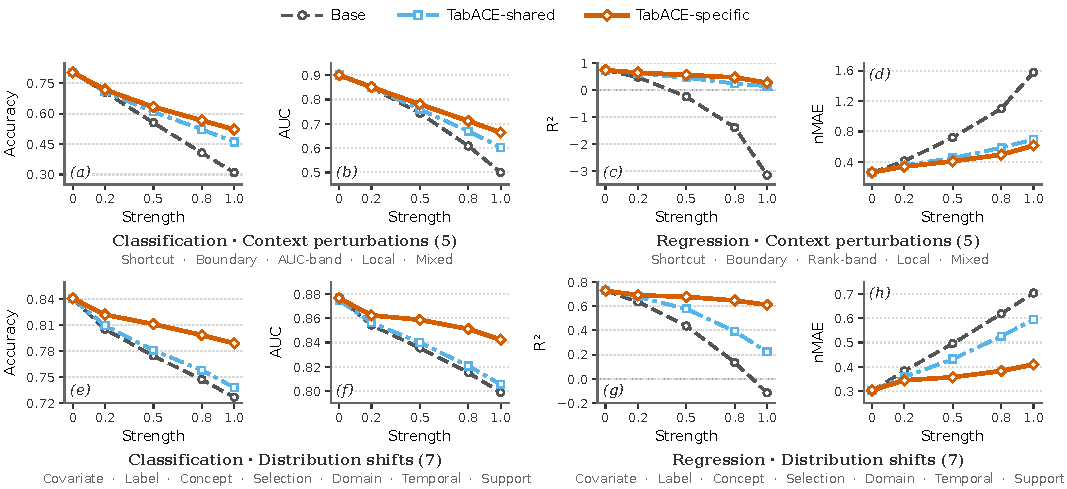
\includegraphics[width=\textwidth]{figures/tabace_strength_comparison.pdf}
  \caption{OpenML 基准上不同问题强度下的性能。分类面板使用 OpenML-CC18，回归面板使用 OpenML-CTR23。第一行对五种受控上下文扰动进行宏平均，第二行对七种分布偏移进行宏平均。}
  \label{fig:semisynthetic-strength}
\end{figure}
\fi

\paragraph{选择方案。}
在每个外层折内，上下文配置、分支权重与整合参数均在其余四个数据集折生成的校准 episode 上拟合，并在留出数据集评估前固定。这些 episode 覆盖已注册的条件，但拟合策略和留出推理均不接收变化强度。所有方法使用相同的外层折与评估样本，留出目标标签仅用于计算最终指标。

% Keep the two compact tables and the inference-cost figure together at the
% top of arXiv page 8, after the page-7 figures and setup text.
\ifdefined\ICLRLayout\else
\clearpage
\definecolor{sharedblue}{RGB}{31,84,147}
\definecolor{specificred}{RGB}{213,94,0}

\begin{table}[H]
  \centering
  \begin{minipage}[t]{0.61\textwidth}
    \vspace{0pt}
    \centering
    \caption{自然地理偏移与时间偏移下的 ID 和 OOD Accuracy。}
    \label{tab:natural-shifts}
    \small
    \setlength{\tabcolsep}{4.0pt}
    \renewcommand{\arraystretch}{1.02}
    \begin{tabular}{@{}llccc@{}}
      \toprule
      方法 & 域 & Employment & Income & TravelTime \\
      \midrule
      \multicolumn{5}{@{}l}{\textit{地理：California $\rightarrow$ Michigan（2018）}} \\
      Base & ID  & 0.7922 & 0.7888 & 0.5912 \\
           & OOD & 0.8043 & 0.7655 & 0.5472 \\
      Shared & ID
        & \textcolor{sharedblue}{0.7948} & \textcolor{sharedblue}{0.7951}
        & \textcolor{sharedblue}{0.5945} \\
           & OOD
        & \textcolor{sharedblue}{0.8078} & \textcolor{sharedblue}{0.7832}
        & \textcolor{sharedblue}{0.5961} \\
      Specific & ID
        & \textcolor{specificred}{\textbf{0.7979}}
        & \textcolor{specificred}{\textbf{0.7955}}
        & \textcolor{specificred}{\textbf{0.6002}} \\
           & OOD
        & \textcolor{specificred}{\textbf{0.8089}}
        & \textcolor{specificred}{\textbf{0.7840}}
        & \textcolor{specificred}{\textbf{0.6034}} \\
      \addlinespace[2pt]
      \multicolumn{5}{@{}l}{\textit{时间：California 2014 $\rightarrow$ 2018}} \\
      Base & ID  & 0.7704 & 0.7926 & 0.5951 \\
           & OOD & 0.7847 & 0.7844 & 0.5908 \\
      Shared & ID
        & \textcolor{sharedblue}{0.7751} & \textcolor{sharedblue}{0.7968}
        & \textcolor{sharedblue}{0.6032} \\
           & OOD
        & \textcolor{sharedblue}{0.7900} & \textcolor{sharedblue}{0.7937}
        & \textcolor{sharedblue}{0.5975} \\
      Specific & ID
        & \textcolor{specificred}{\textbf{0.7757}}
        & \textcolor{specificred}{\textbf{0.7980}}
        & \textcolor{specificred}{\textbf{0.6061}} \\
           & OOD
        & \textcolor{specificred}{\textbf{0.7916}}
        & \textcolor{specificred}{\textbf{0.7947}}
        & \textcolor{specificred}{\textbf{0.5981}} \\
      \bottomrule
    \end{tabular}
  \end{minipage}\hfill
  \begin{minipage}[t]{0.36\textwidth}
    \vspace{0pt}
    \centering
    \caption{上下文集成相对于各未经修改的常规预测器的增益。}
    \label{tab:traditional-backbone-gains}
    \small
    \setlength{\tabcolsep}{4.0pt}
    \renewcommand{\arraystretch}{1.02}
    \begin{tabular}{@{}lcc@{}}
      \toprule
      \multicolumn{3}{c}{分类：$\Delta$Accuracy $\uparrow$} \\
      \cmidrule(lr){1-3}
      预测器 & Shared & Specific \\
      \midrule
      kNN & \textcolor{sharedblue}{+0.0167}
        & \textcolor{specificred}{\textbf{+0.0227}} \\
      Logistic & \textcolor{sharedblue}{+0.0069}
        & \textcolor{specificred}{\textbf{+0.0287}} \\
      CatBoost & \textcolor{sharedblue}{+0.0145}
        & \textcolor{specificred}{\textbf{+0.0287}} \\
      MLP & \textcolor{sharedblue}{+0.0107}
        & \textcolor{specificred}{\textbf{+0.0285}} \\
      \addlinespace[5pt]
      \multicolumn{3}{c}{回归：$\Delta R^2$ $\uparrow$} \\
      \cmidrule(lr){1-3}
      预测器 & Shared & Specific \\
      \midrule
      kNN & \textcolor{sharedblue}{+0.0203}
        & \textcolor{specificred}{\textbf{+0.0654}} \\
      Ridge & \textcolor{sharedblue}{+0.1425}
        & \textcolor{specificred}{\textbf{+0.1966}} \\
      CatBoost & \textcolor{sharedblue}{+0.1279}
        & \textcolor{specificred}{\textbf{+0.1740}} \\
      MLP & \textcolor{sharedblue}{+0.0499}
        & \textcolor{specificred}{\textbf{+0.1645}} \\
      \bottomrule
    \end{tabular}
  \end{minipage}
\end{table}


\begin{figure}[H]
  \centering
  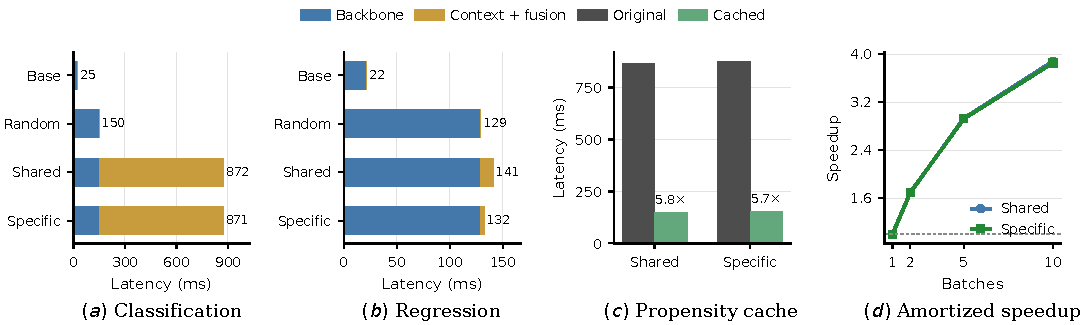
\includegraphics[width=0.96\textwidth]{figures/tabace_inference_cost_ablation.pdf}
  \caption{固定五上下文 Shared 库与单独评估的 Base 分支的推理成本消融。面板 (a--b) 分解中位延迟；(c) 比较原始推理与缓存推理；(d) 在摊销加速比中计入一次性缓存建立成本。}
  \label{fig:inference-cost}
\end{figure}
\fi
